\section{Configuration energy}
Since we have access to various energy parameters for the DDR interface, we will use DDR interface as an example.

\begin{figure}[hbtp]
    \centering
    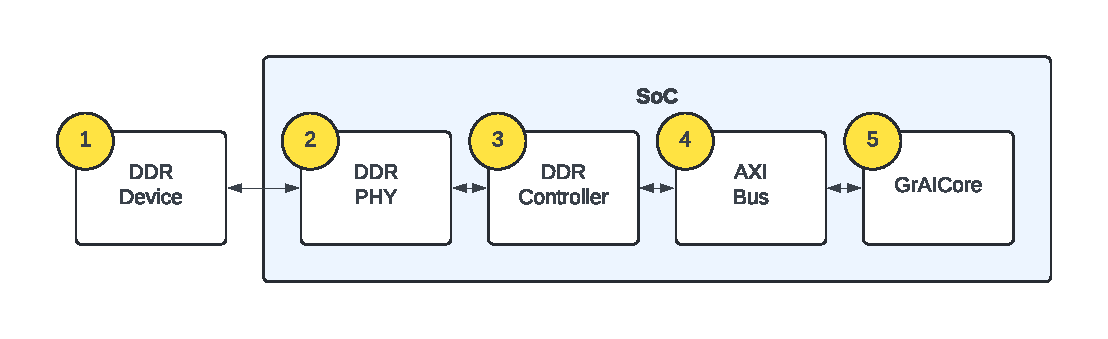
\includegraphics[width=\linewidth]{assets/ddr_graicore_block_diagram.pdf}
    \caption{
        Interconnection of the DDR memory device and \graicore{}
    }
    \label{fig:ddr_graicore_block_diagram}
\end{figure}

% TODO add explanation for every component
% A typical system with DDR as external memory looks as shown in \cref{fig:ddr_graicore_block_diagram}.
% \begin{itemize}
%     \item The \textit{DDR device} where the (model) data is read from.
%     \item The \textit{DDR PHY} that connects the \textit{DDR device} and \textit{DDR controller}.
%     \item The \textit{DDR controller} that handles the read/write requests from the \textit{\graicore{}}.
%     \item The \textit{AXI bus} that connects the \textit{DDR controller} and \textit{\graicore{}}.
%     \item The \textit{\graicore{}} that transfers and writes data the SRAMs.
% \end{itemize}

A typical system with DDR as external memory looks as shown in \cref{fig:ddr_graicore_block_diagram}.
\begin{description}
    \item[Memory device:] 
    The physical component where (model) data is stored and read from.
    This typically takes the form of an integrated circuit that contains an array of memory cells.
    These cells hold individual bits of information, and they are organized into a structured format to allow for efficient access.
    \item[DDR PHY:] 
    A crucial component that bridges the gap between the \graicore{}'s digital signals and the analog signals required by the memory device.
    It manages the high-speed signaling, precise timing, and voltage levels necessary for reliable communication.
    The DDR PHY serializes data from the DDR controller for transmission and deserializes incoming data, ensuring proper data transfer.
    \item[DDR Controller:] 
    This component is responsible for managing all memory operations.
    It acts as an intermediary between the \graicore{} and the memory device, translating the requests from the \graicore{}, such as read and write requests, into the specific control signals required by the memory device.
    The DDR controller also manages essential functions like memory refresh, power management and error correction.
    \item[AXI bus:] 
    The AXI bus (Advanced eXtensible Interface) is a standardized, high-performance interconnect used to connect different components within a SoC.
    It enables parallel data transfer, facilitating high bandwidth and low latency communication between the components.
    Specifically, we explore AXI 4.0.
    \item[\graicore{}:] 
    The major components of the \graicore{} that contributes to the configuration energy is the data transfers through its \confignoc{} and the writing of data to the SRAMs.
\end{description}

For the analysis, we assume that we are using the newly proposed \confignoc{} in \cref{sec:proposed_noc}. 
With the new packet format, a packet contains at most 64 data phits of 64 bits each.
That is, a maximum of 512 bytes\footnote{$64 \times \frac{\SI{64}{b}}{8} = \SI{512}{B}$} of payload per packet.
Furthermore, an additional injection point is introduced (see \cref{fig:segmentation_example_2}).
Next to the injection point connected to the router on the bottom left of the \confignoc{}, a new one is added and connected to the router six positions up.

To estimate the energy cost for configuration, we require the following information from a model:
\begin{itemize}
    \item Amount of data to transfer to the SRAMs
    \item Destination neuron core of the data
\end{itemize}

The amount of data to transfer determines how much data will be read, transferred and written.
We are assuming that the same amount of data read from the external memory is written to the SRAMs.
The location (specific neuron core) of the data determines the amount of hops the data has to perform in the \confignoc{}.
The amount of data to write can also be used to determine the configuration time.
The configuration time is calculated by dividing the amount of data with the write bandwidth.
% The configuration time is used for computing the energy for the \textit{DDR PHY}, \textit{DDR controller} and \textit{AXI bus}.

The amount of data to be written and to which neuron cores depends on how the compiler has performed the mapping on the \graicore{}. % explain
Phits that needs to be transferred to neuron cores further away from an injection point will require more hops to reach, and therefore consume more energy than neuron cores closer to an injection point.
The amount of data that needs to be written to each core differs.
We can retrieve this information from the compiler.

For estimating the energy for the \graicore{} component, we consider the \confignoc{} and the SRAMs.
The \confignoc{} consumes energy by transferring the phits to its destinations via one or multiple hops through the NoC.
The SRAM consumes energy by writing the data to its banks.
A single hop through the \confignoc{} with a 64 bit phit consumes \SI{0.258}{pJ}.
Writing back 64 bits to an SRAM consumes \SI{4.980}{pJ}.

\subsection{Calculation}
The configuration energy consists of the reading, transferring and writing of data from the external memory to the \graicore{}'s SRAMs. 

Let $C$ be the set of tuples holding the coordinates of every core:
\begin{equation*}
    C = \{\,\left(x,y\right) \in \mathbb{N}^2 \mid 1 \leq x \leq 12 \wedge 0 \leq y \leq 11 \,\} 
\end{equation*}

Notice that the x-coordinate and y-coordinate starts at index $1$ and $0$ respectively.

\Cref{fig:model_data_heapmap} shows for a $80\%$ pruned version of ResNet-50\footnote{Internally named \texttt{resnet50\_pruned80\_star}} the amount of data that needs to be written to each of the 144 neuron cores.
We observe that the data is not uniformly distributed across the SRAMs.
Therefore, we require information how much data needs to be transferred to each SRAM.

\begin{figure}[hbtp]
    \centering
    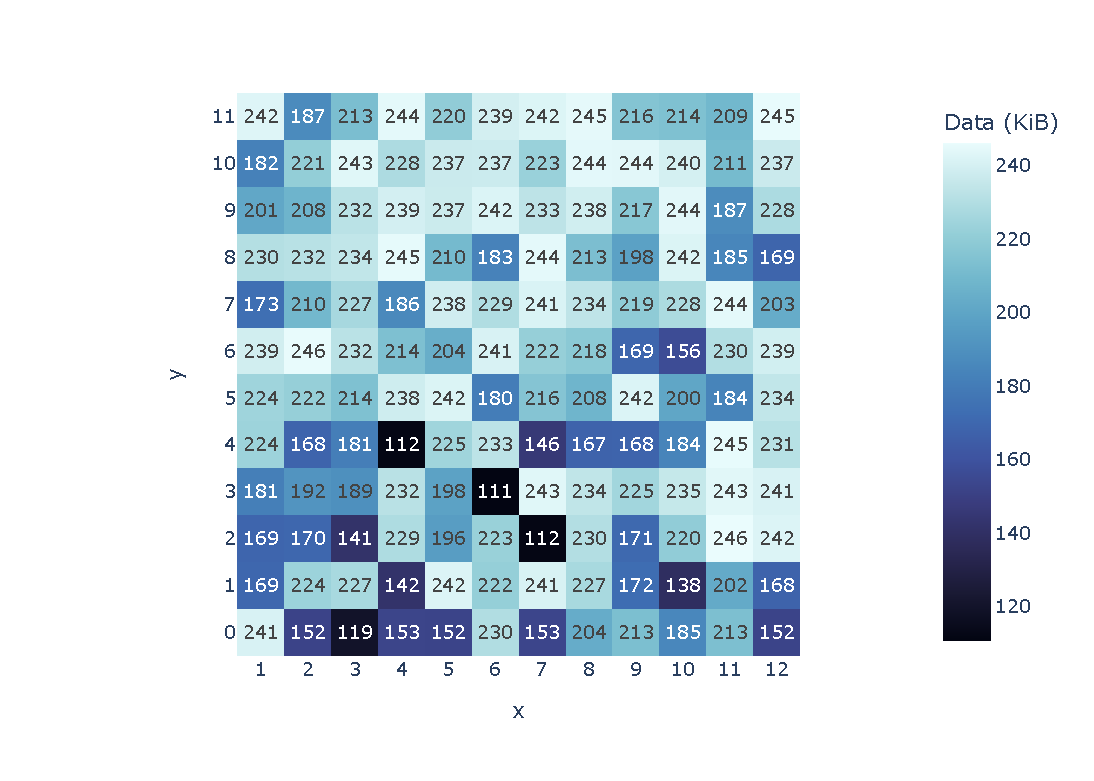
\includegraphics[clip, trim=80 20 10 30, width=0.8\linewidth]{assets/resnet50_coredata_heatmap.pdf}
    \caption{Amount of data to be written to each neuron core for the ResNet-50 model (80\% pruned).}
    \label{fig:model_data_heapmap}
\end{figure}

Let $D$ be a matrix of $12 \times 13$ with $D_{i,j}$ denoting the amount of bytes to be written to core $\left( i,j \right)$.
$D$ has an additional column due to the x-coordinates not starting from index $0$.
Its left-most column is unused (i.e., $D_{0,0}, D_{0,1}, \cdots, D_{0,11}$).
This matrix can be constructed from the artifacts outputted by the compiler.

The number of phits to be transferred through the \confignoc{} influences the total energy costs.
In particular, the amount of phits to be transferred affects the number of hops to be taken in total and the amount of data to be written to the SRAMs.
Therefore, we need to determine how many phits needs to be transferred to each neuron core.
A packet can contain up to 64 data phits, that is $64 \times \SI{64}{b} = \SI{512}{B}$ of payload data.
Suppose we need to transfer $d$ bytes to a neuron core, we then require a total of $\left\lfloor \frac{d}{512} \right\rfloor$ packets with 64 data phits.
If $\left( d \bmod 512 \right) > 0$, then there is an additional packet for the remaining $\left( d \bmod 512 \right)$ bytes of data.
The remaining packet will consist of $\left\lceil \frac{d \bmod 512}{8}\right\rceil$ data phits.
Note that each packet also contains a single phit of 64 bits for the header information.

The total energy cost for configuring the \graicore{} can be estimated with the following equation:
\begin{equation}
    \econf = \eextmem + \enoc + \ewrite
\end{equation}

With:
\begin{align*} 
\eextmem &= 
        \sum_{c \in C}^{}{\ereadextmem(D_c) + \esendtonoc(D_c)} \\
\enoc &=
    \ehop \times \sum_{c \in C}^{}{\nhops(c) \times \ptotal(D_c)} \\
\ewrite &=
    \esramwrite64b \times \sum_{c \in C}^{}{\pdata(D_c)}
\end{align*}

And:
\begin{align*} 
\nhops(x,y) &=
    \begin{cases} 
        x + y & \textrm{if } 0 \leq y \leq 5 \\
        x + y - 6 & \text{if } 6 \leq y \leq 11
    \end{cases}
\\
\ptotal(d) &=
    \left\lfloor \frac{d}{512} \right\rfloor \times (64 + 1) + \left\lceil \frac{d \bmod 512}{8} \right\rceil + 1 =
    \left\lceil \frac{d}{8} \right\rceil + \left\lfloor \frac{d}{512} \right\rfloor + 1 
\\
\pdata(d) &=
    \left\lfloor \frac{d}{512} \right\rfloor \times 64 + \left\lceil \frac{d \bmod 512}{8} \right\rceil =
    \left\lceil \frac{d}{8} \right\rceil
\end{align*}

\begin{eqexpl}[15mm]
    \item{$\ptotal(D_c)$} total phits (includes headers) for transferring $D_c$ bytes
    \item{$\pdata(D_c)$} total data phits (excludes headers) for transferring $D_c$ bytes
    \item{$\nhops(c)$} the amount of hops required to reach a neuron core at coordinate $c$, starting from the router closest to the injection point. It has two sub-functions due to the new \confignoc{}'s dual injector architecture
    \item{$\ereadextmem(D_c)$} energy for reading $D_c$ bytes from the external memory
    \item{$\esendtonoc(D_c)$} energy for sending $D_c$ bytes from the external memory to the \confignoc{}
    \item{$\ehop$} energy for performing a single hop in the \confignoc{}
    \item{$\esramwrite64b$} energy for writing back 64 bits to a neuron core's SRAM
\end{eqexpl}

